%%%%%%%%%%%%%%%%%%%%%%%%%%%%%%%%%%%%%%%%%%%%
% Submitted Abstract

%The deep chlorophyll maximum (DCM) is a well known feature of the global ocean. However, its description and the study of its formation are a  challenge, especially in the peculiar environment that is the Black Sea. The retrieval of chlorophyll a (Chla) from fluorescence (Fluo) profiles recorded by biogeochemical-Argo (BGC-Argo) floats is not trivial in the Black Sea, due to the very high content of colored dissolved organic matter (CDOM) which contributes to the fluorescence signal and produces an apparent increase of the Chla concentration with depth.

%Here, we revised Fluo correction protocols for the Black Sea context using co-located in-situ high-performance liquid chromatography (HPLC) and BGC-Argo measurements. The processed set of Chla data (2014–2019) is then used to provide a systematic description of the seasonal DCM dynamics in the Black Sea and to explore different hypotheses concerning the mechanisms underlying its development.

%Our results show that the corrections applied to the Chla profiles are consistent with HPLC data. In the Black Sea, the DCM begins to form in March, throughout the basin, at a density level set by the previous winter mixed layer. During a first phase (April-May), the DCM remains attached to this particular layer. The spatial homogeneity of this feature suggests a hysteresis mechanism, i.e., that the DCM structure locally influences environmental conditions rather than adapting instantaneously to external factors.

%In a second phase (July-September), the DCM migrates upward, where there is higher irradiance, which suggests the interplay of biotic factors. Overall, the DCM concentrates around 45 to 65% of the total chlorophyll content within a 10 m layer centered around a depth of 30 to 40 m, which stresses the importance of considering DCM dynamics when evaluating phytoplankton productivity at basin scale.

%%%%%%%%%%%%%%%%%%%%%%%%%%%%%%%%%%%%%%%%%%%%

\documentclass[final]{beamer}
%% Possible paper sizes: a0, a0b, a1, a2, a3, a4.
%% Possible orientations: portrait, landscape
%% Font sizes can be changed using the scale option.
\usepackage[size=a0,orientation=landscape,scale=1.25]{beamerposter}
\usetheme{ARTMAN_PERSEUS}
%\usetheme{LLT-poster}
%\usecolortheme{ComingClean}
%\usecolortheme{Entrepreneur}
%\usecolortheme{ConspicuousCreep}  %% VERY garish.

\usepackage[utf8]{inputenc}
\usepackage[T1]{fontenc}
\usepackage{libertine}
\usepackage[scaled=0.92]{inconsolata}
% \usepackage[libertine]{newtxmath}

\graphicspath{{./figs/}
  {./figs/logo/}
}


\author[acapet@ulg.ac.be]{Arthur Capet$^1$, Audrey Plante$^2$, Lei Chou$^2$, Nathalie Fagel$^3$, Adrian Teaca$^4$, and Marilaure Grégoire$^1$}
\title{Biogeochemical controls on the Black Sea oxygen dynamics}
\subtitle{Relevant diagnostics, key processes and adequacy of the monitoring infrastructure}

\institute{
  $^1$ Modeling for aquatic systems (MAST), ULiege, Belgium
  }
  
% Optional foot image
% \footimage{           
\includegraphics[width=9cm]{mast.png}
%            \vspace{1cm}
%                       \includegraphics[width=7cm]{uliege.jpg}
%            \vspace{3cm}
%             }

\begin{document}
  \begin{frame}[fragile]\centering
    
    \begin{columns}[T]
      
      %%%%%%%%%%%%%%%
      % LEFT COLUMN %
      %%%%%%%%%%%%%%%   
      
      \begin{column}{.33\textwidth}
	\section{Context \& Method}
%	\subsection{Deep Chlorophyll Maximum}
	%%% CONTEXT
	\begin{block}{Deep Chlorophyll Maximum (DCM)}
% 	  To resolve the \alert{role and response} of \alert{macrobenthos} in coastal \alert{hypoxia} dynamics
% 	  \vskip 5mm
% 	      \begin{figure}
% %		\includegraphics[width=.9\columnwidth]{B8_ext}
% 	      \end{figure}

% 	  \begin{columns}[T]
% 	    \begin{column}{.5\columnwidth}	  
% 	      Work hypotheses
% 	      \begin{itemize}
% 		\item \alert{[$O_2$]} shapes the distribution of \alert{benthic populations \& activity}
% 		\item  \alert{Macrobenthic activity} affects \alert{Benthic-Pelagic coupling}
% 	      \end{itemize}
% 	    \end{column}
% 	    \begin{column}{.5\columnwidth}	  
% 	      Assumptions to conciliate spatial scales
% 	      \begin{itemize}
% 		\item We use \alert{functional traits} to synthetize macrobenthic activity
% 		\item We use \alert{bentic meta-models} to represent diagenesis in a 3D model
% 	      \end{itemize}
% 	    \end{column}	
% 	  \end{columns}
	\end{block}
	
	\begin{block}{BGC-Argo}
	   dd
	\end{block}

	  

	
% 	%%%% APPROACH
% 	\begin{block}{Methodology}
% 	  \begin{figure}
% %	    \includegraphics[width=.8\columnwidth]{ExecScheme}
% 	  \end{figure}
% 	\end{block}
	
	%% CONCLUSIONS & Persepectives
	\section{Conclusions \& Perspectives}
	\begin{alertblock}{Conclusions}
	%  	  \vskip -5mm
%	  \begin{columns}[T]
%	    \begin{column}{.63\columnwidth}	  
	      \begin{itemize}
		    \item 
	        \item 
	        \item 
	      \end{itemize}
	\end{alertblock}
	
	\begin{block}{Further Readings}
	%  	  \vskip -5mm
%	  \begin{columns}[T]
%	    \begin{column}{.63\columnwidth}	  
	      \begin{itemize}
		    \item 
	        \item 
	        \item 
	      \end{itemize}
	\end{block}
	
	%% REFS
	\begin{block}{References}
	%  \vskip -5mm
	  \footnotesize
	  \begin{description}
	    \item[1] Capet, A., Meysman, F. J. R., Akoumianaki, I., Soetaert, K. \& Grégoire, M. Integrating sediment biogeochemistry into 3D oceanic models: a study of benthic-pelagic coupling in the Black Sea. Ocean Model. (2016).
	    \item[2] Soetaert, K., Middelburg, J. J., Herman, P. M. J. \& Buis, K. On the coupling of benthic and pelagic biogeochemical models. Earth-Sci. Rev. 51, 173–201 (2000).
	    \item[3] Wijsman, J. W. M., Herman, P. M. J. \& Gomoiu, M. T. Spatial distribution in sediment characteristics and benthic activity on the northwestern Black Sea shelf. Mar. Ecol. Prog. Ser. 181, 25–39 (1999).	  \end{description}
	\end{block}
      \end{column}
      
      %%%%%%%%%%%%%%%%%
      % SECOND COLUMN % 
      %%%%%%%%%%%%%%%%%
      
      %%% RESULTS 
      \begin{column}{.64\textwidth}
       \section{Results}
      

	%%%% COMP MODELS 
	\begin{block}{Morphology of Chl profiles}
	 % \vskip -12mm
	Chl profiles recalibrated from BGC-Argo fluorescence data are classified in terms of best-matching analytic forms. 
	  \begin{columns}[T]
	    \begin{column}{.32\textwidth}
	    \centering{\alert{ Non-DCM profiles}}
	   

	    \end{column}
	    
	    \begin{column}{.32\textwidth}
	      \begin{figure}
     		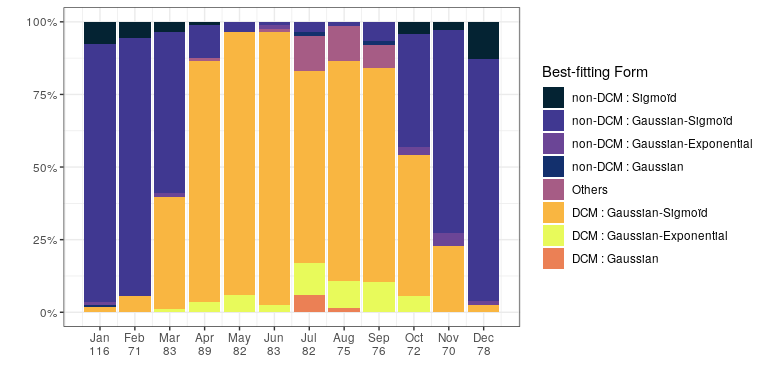
\includegraphics[height=13cm]{figs/FIG3.png}
	  	   %   \caption*{ \centering Calibration identifies \alert{probability distributions} for parameters of the OMEXDIA diagenetic model  (Here: Station 6, Emblas 2016 Campaign)}  
		    \end{figure}
	    \end{column}
	  
	    \begin{column}{.32\textwidth}
	       \centering{\alert{DCM profiles}}
	      
	    \end{column}	    
	  \end{columns}
	  	  \vskip -5mm
	\end{block}
	
	%%%% META
	\begin{block}{ Macrobenthic Facies $\rightarrow$ Meta-Models for Benthic-Pelagic Coupling }
	  	  \vskip -12mm
	  \begin{columns}[T]
	    \begin{column}{.30\textwidth}
	      \begin{figure}
%		\includegraphics[height=12cm]{pdenit2_explain}
		\caption*{\footnotesize \alert{pdenit}: Part of benthic respiration led by denitrification. \alert{Cmin}: Carbon mineralized per unit of time. \alert{bwO2}: Bottom Oxygen concentration.
	      Other dimensions are not represented.}
	      \end{figure}
	    \end{column}
	    
	    \begin{column}{.40\textwidth}
	      \justify
	      \alert{\textbf{$\leftarrow$}} 
	      The \alert{1D diagenetic model} is run multiples times while perturbing \alert{Bottom water nutrients and organic input} within ranges obtained from 3D simulations
		, and \alert{Macrobenthic activity parameters} within ranges obtained during calibrations.\\	
	      Those simulations are used to adjust meta-model functions, that are implemented in the 3D water-column model to represent the behavior of the 1D diagenetic model. \\
	      \vspace{15mm}
	      
	      Set of functions are issued for different facies of macrobenthic  \alert{$\rightarrow$}  
	      activity, to be used for different regions of the 3D model.      
	    \end{column}


	    \begin{column}{.30\textwidth}
	      \begin{figure}
%		\includegraphics[height=16cm]{AllMeta}
	      \end{figure}
	    \end{column}
	  \end{columns}
	  \vskip -5mm
	\end{block}
	
	%%%% 1D - 3D
	\begin{block}{Benthic-Pelagic coupled simulations 1D \& 3D}
	   \vskip -12mm
	  \begin{columns}[T]
	    
	    \begin{column}{.30\textwidth}
	      \begin{figure}
%		\includegraphics[height=17cm]{FinalFL}
	      \end{figure}
	    \end{column}
	    
	    \begin{column}{.18\textwidth}
	      \justify
	      \alert{\textbf{$\leftarrow$}} 
	      The sensitivity of Benthi-Pelagic coupling is explored with  \alert{1D simulations}, for typical shelf conditions.  \\
	      To mitigate the lack of lateral flows, a weak relaxation towards 3D model outputs is imposed. \\
	      The three simulations shown here differ only in terms of macrobenthic facies (see above). 
	    \end{column}

	    \begin{column}{.02\textwidth}
	    
	    \end{column}
	    
	    \begin{column}{.25\textwidth}
	      \begin{figure}
%		\includegraphics[width=\columnwidth]{SedModel}
	      \end{figure}
	   \alert{ 3D simulations} resolve the coupled dynamics of the Black Sea north western shelf. 
	    Those are used to reproduce the diversity of benthic-pelagic coupling (above) and the dynamics of seasonal hypoxia (right).
	    \end{column}
	    
	    \begin{column}{.30\textwidth}
	      \begin{figure}
%		\includegraphics[height=18cm]{MonthlyClim_O2bottomSHELF}
	      \end{figure}
	    \end{column}
	    
	  \end{columns}
	  	  \vskip -5mm
	\end{block}
	
      \end{column}
    \end{columns}
    
    % \vspace{2cm}
    % \begin{columns}[T]
    % \end{columns}
    
    
\end{frame}
\end{document}